\chapter{Results}

To properly contextualize the results, we begin by briefly presenting the initial data.

The relative production quantiles, which were used to segment the other time series, are illustrated as follows:

\begin{figure}[!h]
	\centering
	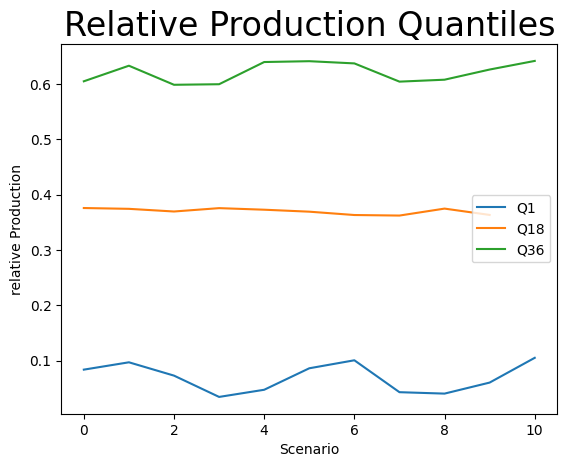
\includegraphics[width=0.7\linewidth]{pictures/results/relativeProduktionQuantils.png}
	\caption{Relative Production Quantiles}
	\label{fig:Relative Production Quantiles}
\end{figure}

Based on these, the resulting time series for activated balancing energy and their corresponding prices are shown below:
The corresponding data for the aFFR market is presented in the Appendix~\ref{chap:app_QaFFRmarketData}
The data indicate that, with increasing market penetration of volatile energy sources, the volume of activated negative balancing energy increases,
whereas the demand for positive balancing energy tends to decrease.
A similar pattern emerges in the marginal prices for activated balancing energy.
While the prices for negative balancing energy rise with a higher share of volatile producers,
the prices for positive balancing energy decline.
Notably, there are significant outliers in the time series of marginal prices for positive balancing energy,
especially in scenarios with medium and low market penetration of volatile producers.

The median balancing capacity prices peak for
both negative and positive in the medium volatility scenario.
In the first quantile's data, the prices for negative capacity are comparable to those in the 36th quantile.
For positive balancing energy, however, the 36th quantile diverges significantly from the 1st quantile,
especially during the later hours of the day.

Based on these time series, the model produced the following results:

The bidding strategy for capacity market prices consistently remains just below the expected marginal price across all scenarios.
The optimization selects a bid price equal to 90\% of the expected marginal market price.

It can be observed that the provision of negative balancing energy occurs earlier in the low and medium scenarios
when both balancing power bids are accepted [Figure \ref{fig:Negative Balance Energy - Q1}, \ref{fig:Negative Balance Energy - Q18}].
This temporal shift is not observed in scenarios with high volatility energy production penetration [Figure \ref{fig:Negative Balance Energy - Q36}].

While the bidding quantities for positive balancing energy remain largely consistent across low and medium volatility scenarios,
regardless of capacity market acceptance, more pronounced differences appear under high-volatility conditions.
In these scenarios, earlier energy provision also results from tighter restrictions due to capacity market results.

To aid in interpretation, we define the following restriction categories:
\begin{enumerate}
	\item Restricted: B $\rightarrow$ RL accepted for both input and output (blue)
	\item Restricted: O $\rightarrow$ RL accepted for output, declined for input (orange)
	\item Restricted: I $\rightarrow$ RL accepted for input, declined for output (green)
	\item Restricted: N $\rightarrow$ RL declined for both input and output (red)
\end{enumerate}

The results indicate a relatively consistent bidding behavior in the capacity market across all scenarios.

\begin{figure}[!h]
	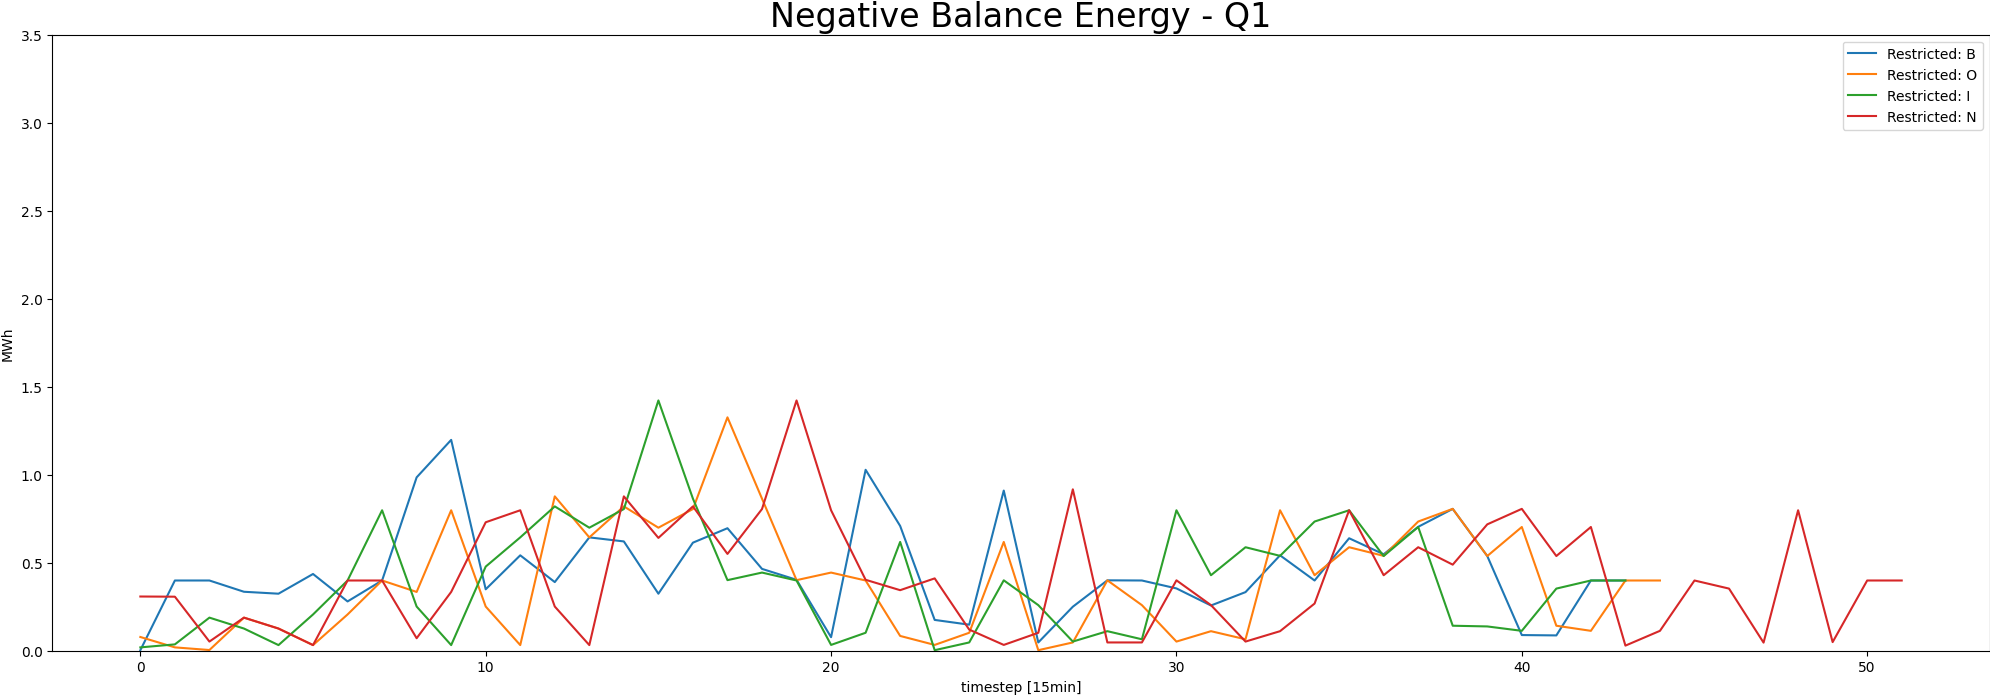
\includegraphics[width=1\linewidth]{pictures/results/Negative Balance Energy - Q1.png}
	\caption{Negative Balance Energy - Q1}
	\label{fig:Negative Balance Energy - Q1}
\end{figure}

\begin{figure}[!h]
	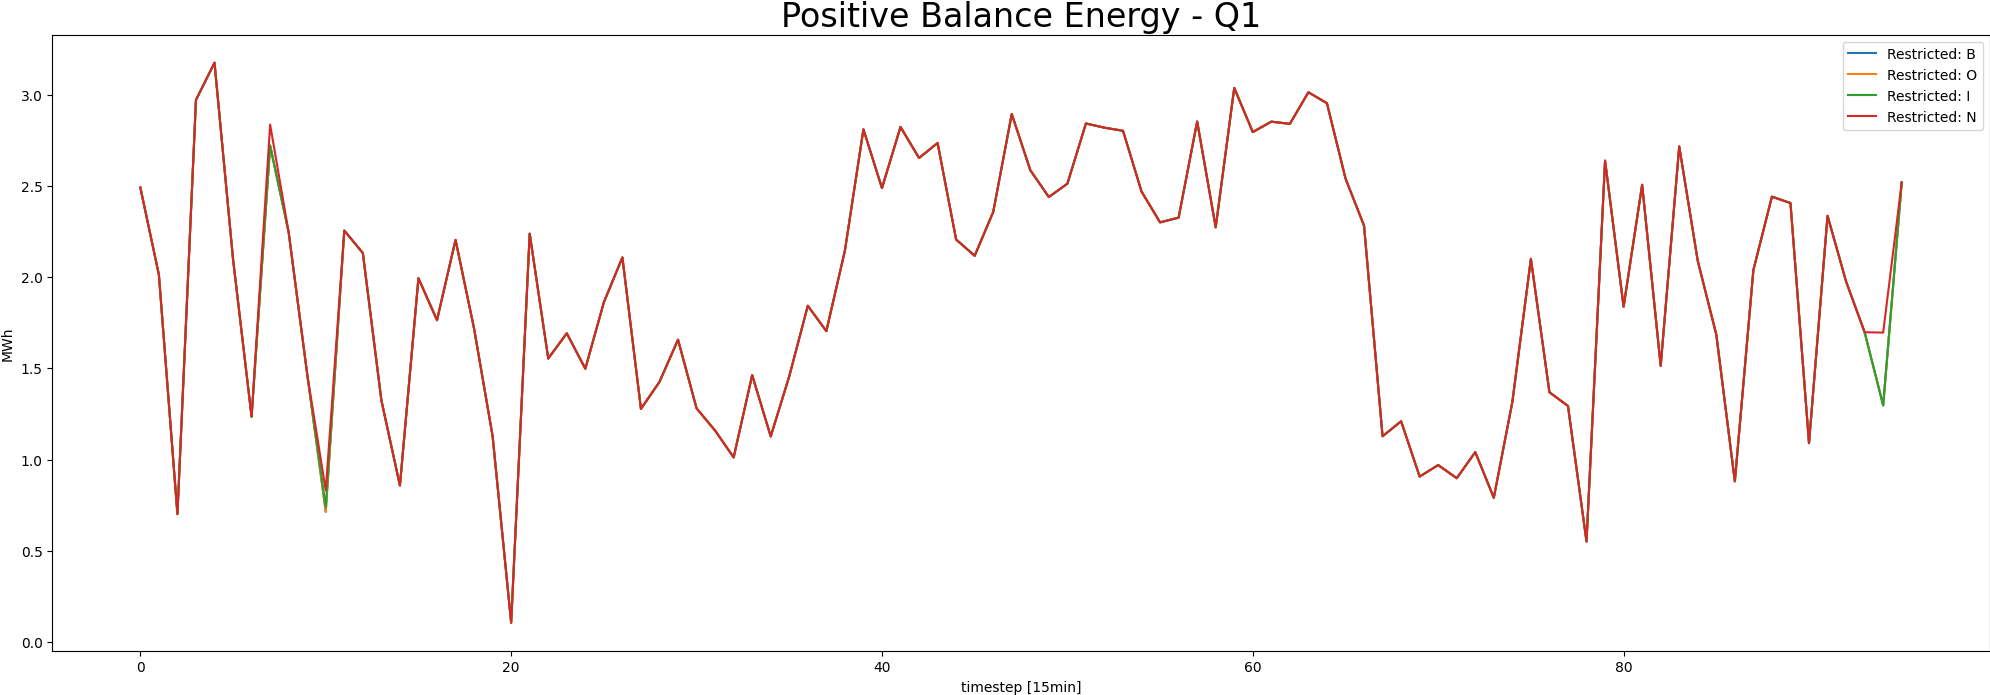
\includegraphics[width=1\linewidth]{pictures/results/Positive Balance Energy - Q1.png}
	\caption{Positive Balance Energy - Q1}
	\label{fig:Positive Balance Energy - Q1}
\end{figure}

\begin{figure}[!h]
	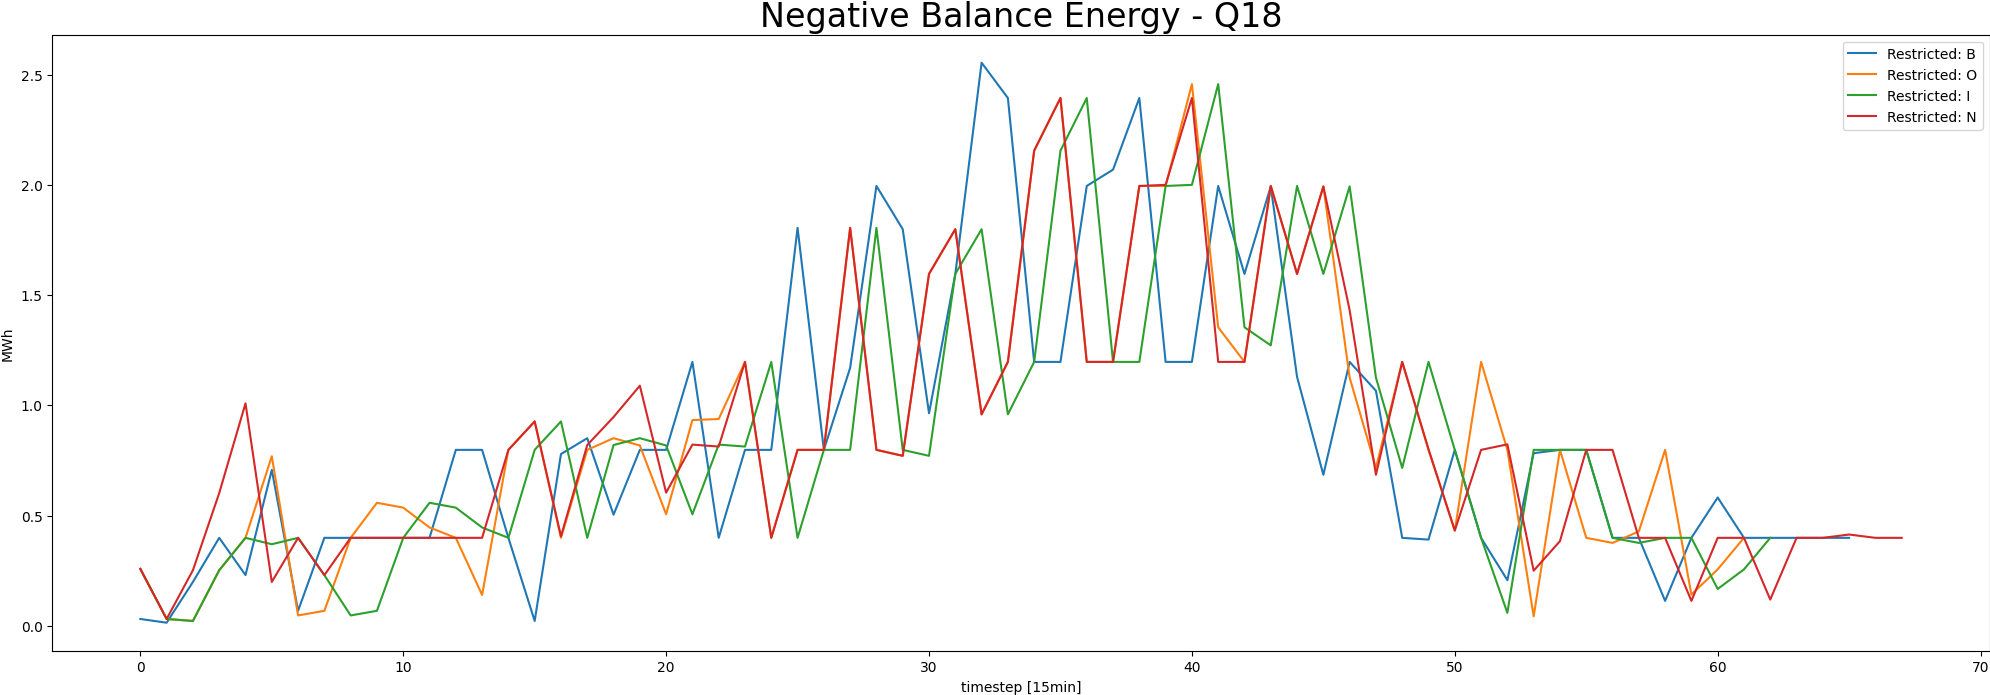
\includegraphics[width=1\linewidth]{pictures/results/Negative Balance Energy - Q18.png}
	\caption{Negative Balance Energy - Q18}
	\label{fig:Negative Balance Energy - Q18}
\end{figure}

\begin{figure}[!h]
	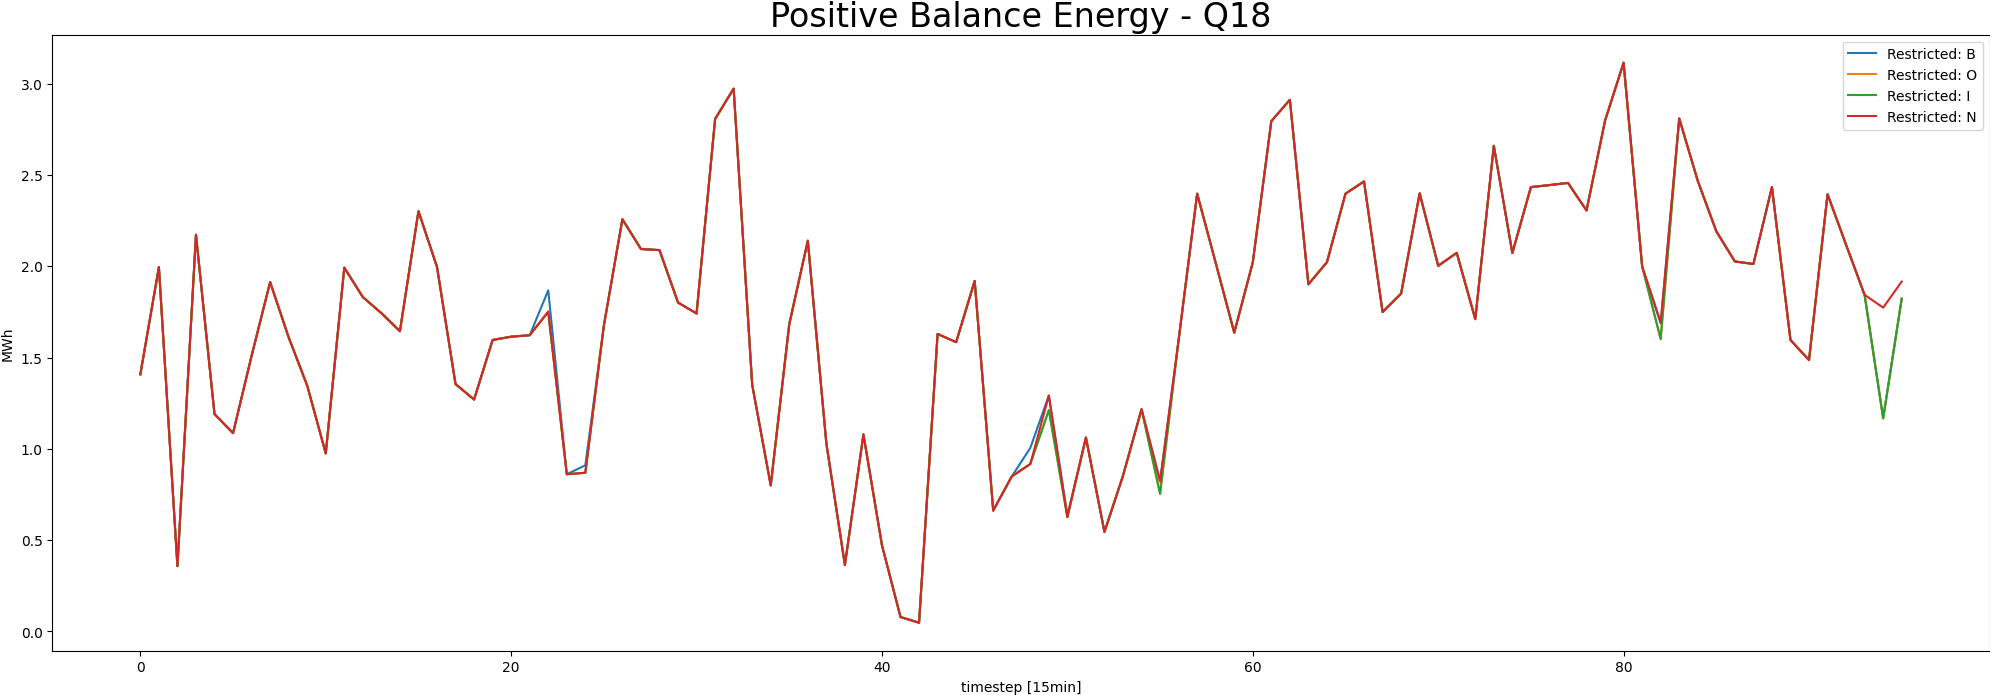
\includegraphics[width=1\linewidth]{pictures/results/Positive Balance Energy - Q18.png}
	\caption{Positive Balance Energy - Q18}
	\label{fig:Positive Balance Energy - Q18}
\end{figure}

\begin{figure}[!h]
	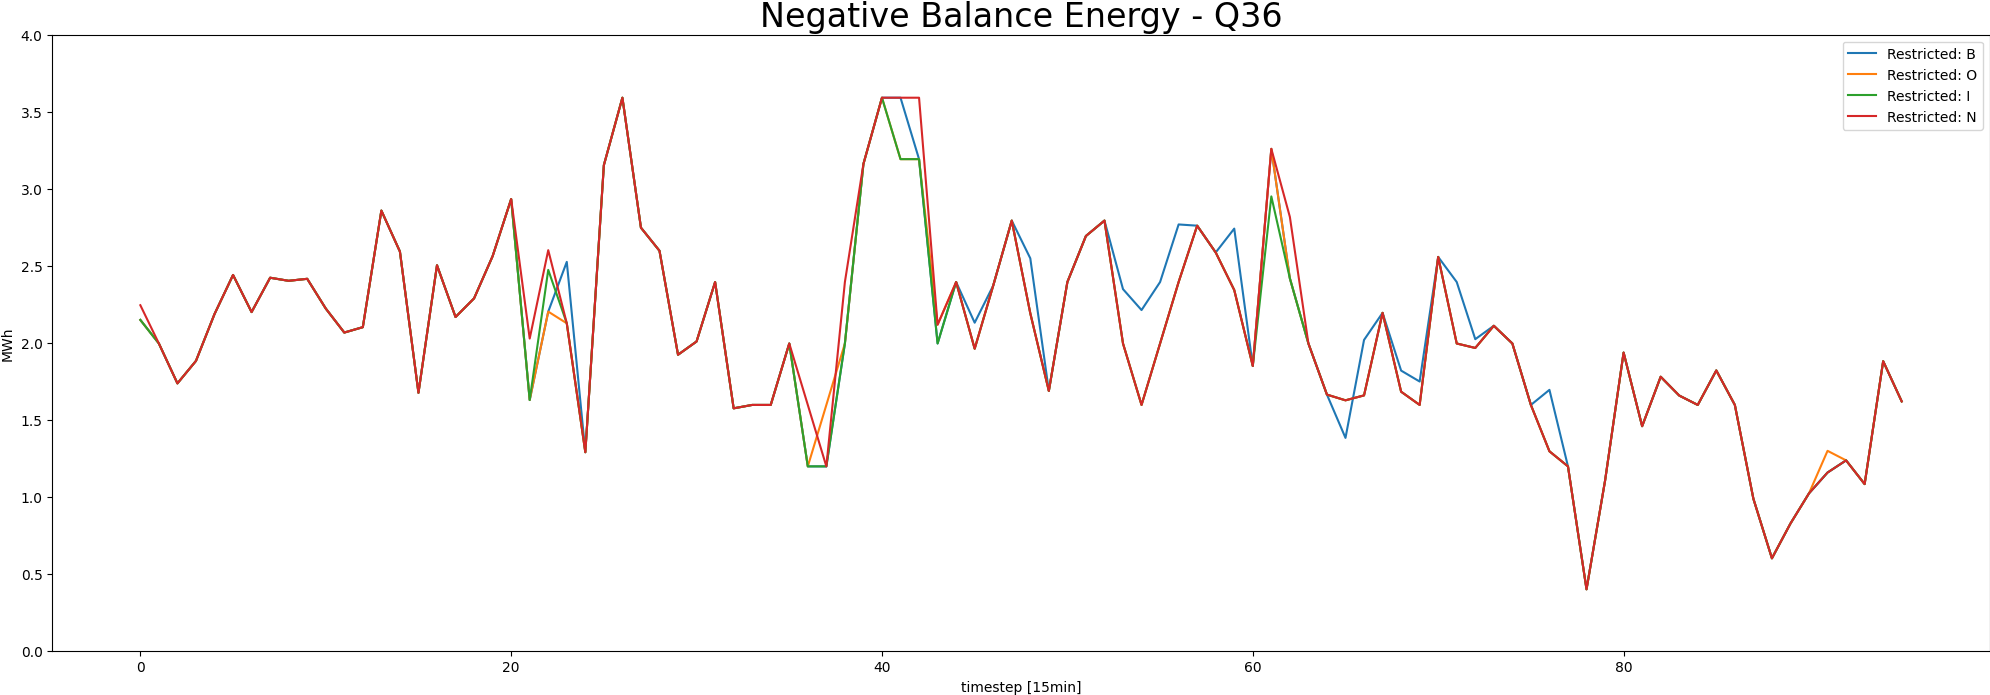
\includegraphics[width=1\linewidth]{pictures/results/Negative Balance Energy - Q36.png}
	\caption{Negative Balance Energy - Q36}
	\label{fig:Negative Balance Energy - Q36}
\end{figure}

\begin{figure}[!h]
	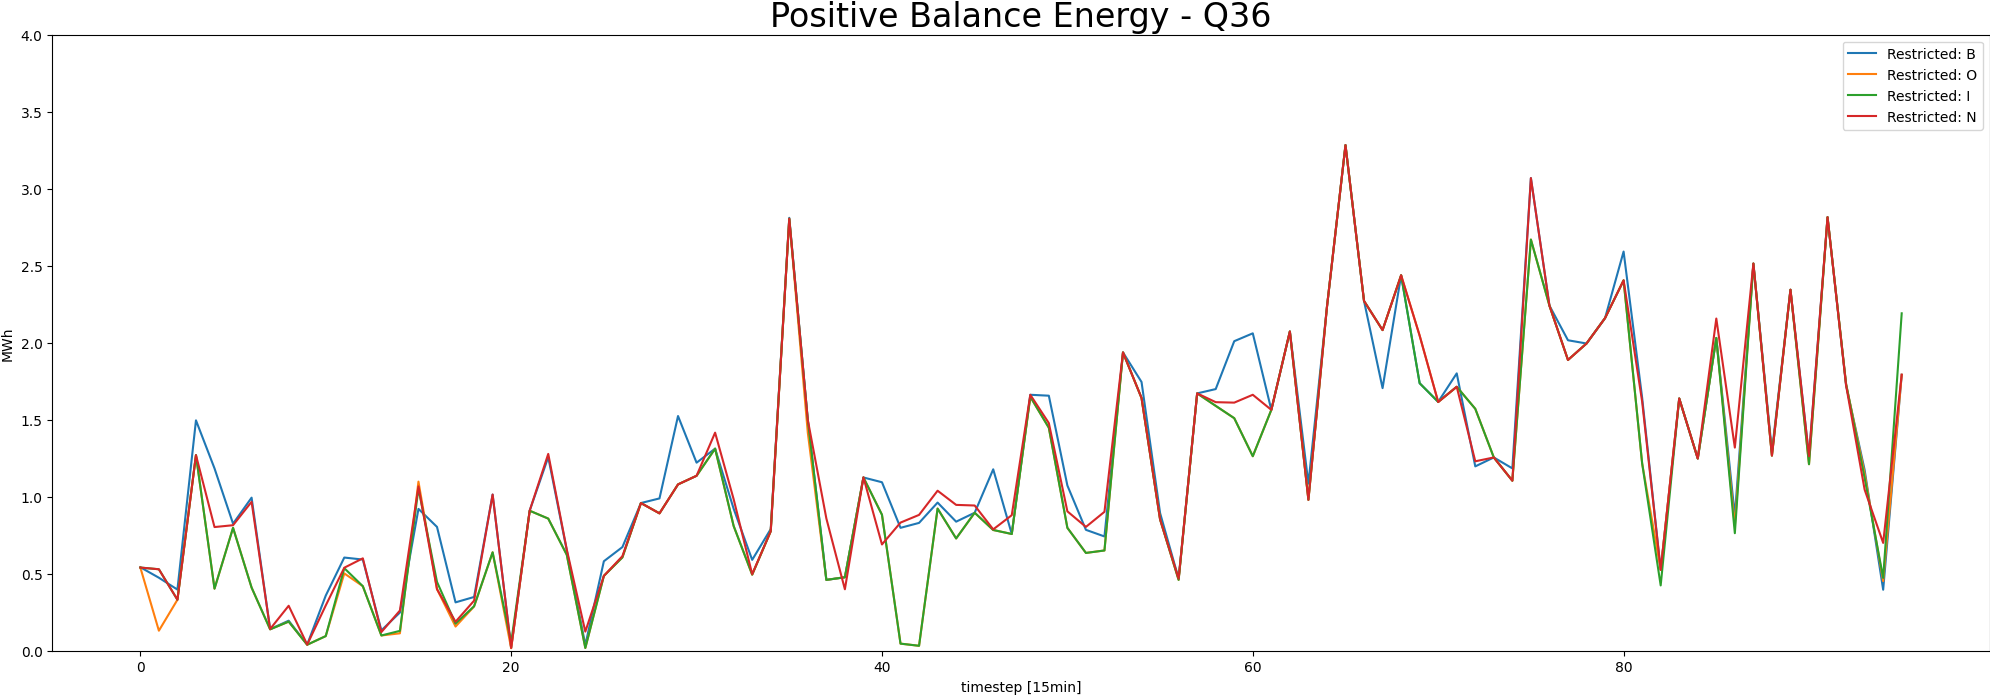
\includegraphics[width=1\linewidth]{pictures/results/Positive Balance Energy - Q36.png}
	\caption{Positive Balance Energy - Q36}
	\label{fig:Positive Balance Energy - Q36}
\end{figure}
